\documentclass{article}

% Language setting
% Replace `english' with e.g. `spanish' to change the document language
\usepackage[english]{babel}

% Set page size and margins
% Replace `letterpaper' with `a4paper' for UK/EU standard size
\usepackage[a4paper]{geometry}

% Useful packages
\usepackage{amsmath}
\usepackage{graphicx}
\usepackage[colorlinks=true, allcolors=blue]{hyperref}

\title{Intro to Machine Learning - HW 01}
\author{Galit Dotan}
\date{\today}

\begin{document}
    \maketitle


    \section{Visualizing the Hoeffding Bound}\label{sec:visualizing-the-hoeffding-bound}

    \begin{figure}[htp]
        \centering
        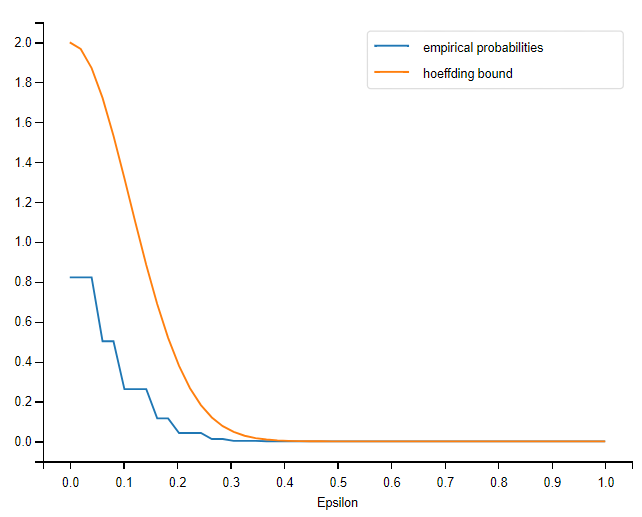
\includegraphics{images/Hoeffding}
        \caption{\label{fig:hoeffding}Hoeffding Bound Results}
    \end{figure}

    \newpage


    \section{Nearest Bound}\label{sec:nearest-bound}

    \subsection{Results with n=1000; k=10}\label{subsec:results-with-n=1000;-k=10}

    The accuracy percentage is \textbf{85.8\%}.

    Note that for a completely random predictor we would expect the accuracy to be around 10\% (for each test there are 10 possible predictions (the digits 0 to 9) - only one of them is correct. So there is a 10\% chance of guessing the correct one).

    Our kNN's prediction for n=1000 and k=10 is better than this, which means that it was able to learn.

    \subsection{Prediction accuracy as a function of k}\label{subsec:prediction-accuracy-k}

    \begin{figure}[htp]
        \centering
        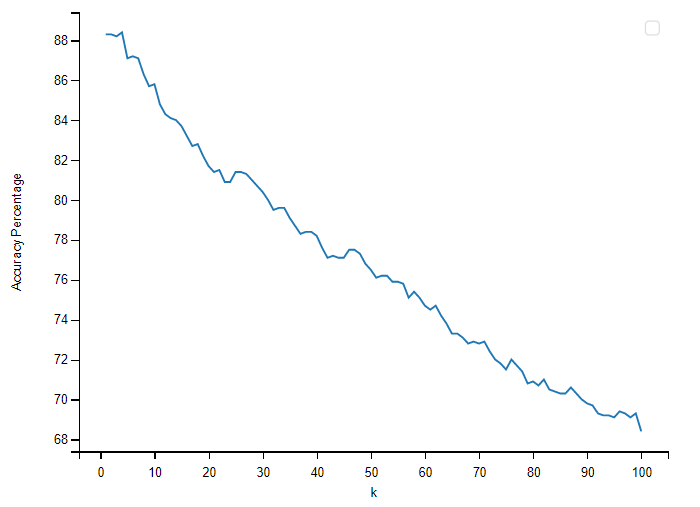
\includegraphics{images/q_2c}
        \caption{\label{fig:k-results}Accuracy Per-k Results}
    \end{figure}

    \subsubsection{Discussion}

    Best value was received for k is \textbf{k=4}: 88.4\%.

    Note that the larger the k is - the algorithm takes into consideration the labels of more images.
    Given that the images are ordered from most similar to k to least similar - the higher k is, the more distant images are taken into consideration.

    This is especially true, given the fact that n=1000 is a rather small train set.

    Assuming there is an equal distribution of the digits 0--9 in the full dataset, for each image chosen to the train subset of the dataset, there is a 1/10 chance to choose each digit.

    For example, for k=100, the k nearest neighbors are $1/10$ - which is a lot.

    \subsection{Prediction Accuracy Per different n Sizes}

    \begin{figure}[htp]
        \centering
        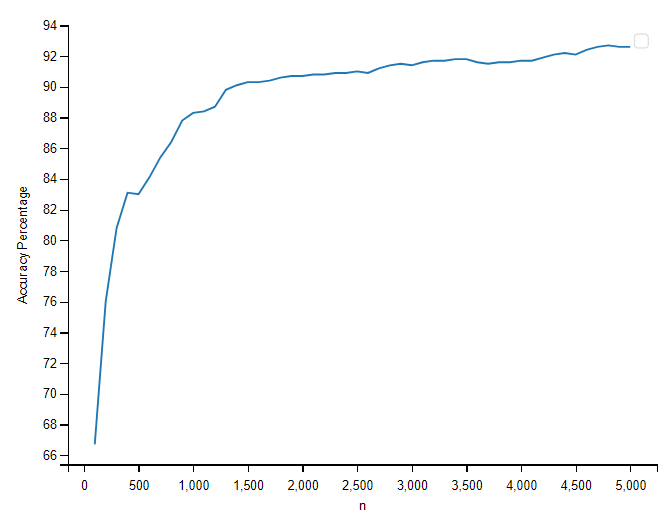
\includegraphics{images/q_2d}
        \caption{\label{fig:n-results}Accuracy Per-n Results}
    \end{figure}

\end{document}